besoin en entrée à méthode « agile » - \\
description de la méthode – \\
application et différence par rapport // DTI +\\
enrichir le produit si cela marche\\
Avantage/inconvénient Extreme programming :\\
Revue logicielle (validations qui permettront de faire évoluer le produit)

\section{La méthodologie appliqué}
Pour la réalisation de ce projet, vue les circonstance, une méthodologie existante c'est mise en place automatiquement. Celle ci est l'Extreme programming\footnote{L'Extreme Programming a été inventée par Kent Beck, Ward Cunningham et Ron Jeffries pendant leur travail sur un projet « C3 » de calcul des rémunérations chez Chrysler. Kent Beck, chef de projet en mars 1996 commença à affiner la méthodologie de développement utilisée sur le projet. La méthode est née officiellement en octobre 1999 avec le livre Extreme Programming Explained de Kent Beck. "Wikipedia"} décrite ci-après.

Dans les méthodes traditionnelles, les besoins sont définis et souvent fixés au départ du projet informatique ce qui accroît les coûts ultérieurs de modifications. Extreme programming s'attache à rendre le projet plus flexible et ouvert au changement en introduisant des valeurs de base, des principes et des pratiques.

L'Extreme Programming repose sur des cycles rapides de développement (des itérations de quelques semaines voir dans notre cas quelques jours seulement) dont les étapes sont les suivantes:
\begin{itemize}
\item une phase d'exploration détermine les scénarios clients qui seront fournis pendant cette itération,
\item la transformation des scénarios en tâches à réaliser et en tests fonctionnels,
\item lorsque tous les tests fonctionnels passent, le produit est livré.
\end{itemize}
..
Lorsqu'une tâche est terminée, les modifications sont immédiatement intégrées dans le produit complet. On évite ainsi la surcharge de travail liée à l'intégration de tous les éléments avant la livraison. Les tests facilitent grandement cette intégration: quand tous les tests passent, l'intégration est terminée.

Le cycle se répète tant que le client peut fournir des scénarios à livrer (cf. Fig. \vref{XP}). Généralement le cycle de la première livraison se caractérise par sa durée et le volume important de fonctionnalités embarquées. Après la première mise en production, les itérations peuvent devenir plus courtes (par exemple la séparation des plans de vol en catégories tel que: transit, interne …)
\begin{figure}
\center
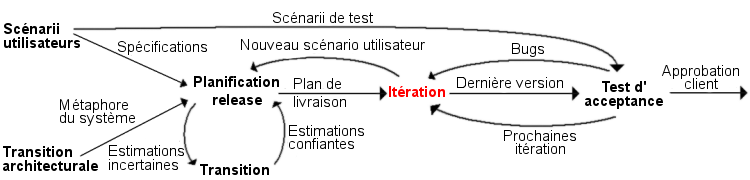
\includegraphics[width=15cm]{images/xp.png}
\caption{Cycle de l'Exreme Programing.}
\label{XP}
\end{figure}
